\chapter{Introduction}
\label{chapter:introduction}

\section{Overview of the problem}

In recent years, interest in the field of artificial intelligence has boomed, both among the public and among researchers. In 2022, the number of publications related to AI was nearly triple that of ten years prior \cite{Nestor:2024}. However, most of this research appears to focus mainly on the accuracy of the AI models, with only a small percentage of papers being dedicated to or giving similar importance to their efficiency \cite{Schwartz:2019}.

By 2018, the computing cost of some of the biggest deep learning models had increased by a factor of over 3.000.000 compared to six years before \cite{Amodei:2018}, and the doubling period for that cost is still estimated to be less than a year \cite{Jaime:2022}. When considering that the energy consumed often comes from non-renewable and carbon-positive sources \cite{Strubell:2019}, the impact that the industry has on the environment cannot be overlooked.

In the case of reinforcement learning, one of the biggest factors that increases the training costs is the complexity of the environment that the model has to learn. As the number of possible states and actions increases, and especially if the results of the actions are non-deterministic or there are other elements outside of the agent's control that can affect the environment, the difficulty of training and tuning RL models skyrockets. A potential solution to that problem can be found in hierarchical reinforcement learning, a methodology that consists of subdividing the main goal of the environment into several subtasks and training smaller specialized agents for each of the tasks \cite{Barto:2003, Al-Emran:2015, Pateria:2021}. Our hypothesis is that this approach can be used in complex environments to achieve solutions with equal or greater performance than traditional reinforcement learning with a smaller compute cost, which translates into less energy consumption and less carbon emissions.

\section{Personal motivation}

My particular motivation to work on this project is twofold. On one hand, and like many people, I am quite concerned about the current trend of global warming and the grim outlook for the environment in the coming decades. As such, taking part in a project aimed at finding solutions to reduce carbon emissions aligns strongly with my values.

On the other hand, I see this as an opportunity to further study and learn about the topic of reinforcement learning. I was already very interested in RL before beginning my studies in this Master's course, and that interest has only grown as I have learned more about the topic. For this project, I am excited to work on hierarchical reinforcement learning as a particular branch of the broader discipline.

\section{Goals}
\label{section:goals}

In this thesis, we will continue the work of prior students \cite{Caceres:2024, Gimenez:2024} in determining whether a hierarchical assembly of specialized agents can be used to achieve comparable results to a single agent while generating less carbon emissions during training. In the previous work, it was established that the multi-agent strategy was able to achieve better performance and greater consistency than the single agent, but not with a smaller energy consumption.

The main goal of the project will be to find under what conditions a multi-agent strategy can outperform a single agent in both performance and training efficiency. The following is the list of subgoals we have chosen that will help us reach the main goal:

\begin{itemize}
    \item \textbf{Reducing built-in logic in actions.} In the previous environment, actions had a considerable amount of pre-programmed logic to simplify and streamline the action space. We believe this might have allowed a single agent, and even a random agent, to compete more closely with the hierarchical agent, which should fair better with a more complex action space.
    \item \textbf{Improving the reward signal.} We believe there is still room to improve when it comes to the default reward signal provided by the environment and the custom reward used in the previous work.
    \item \textbf{Finding new subtasks.} The strength of the hierarchical strategy rests in dividing the main objective of the environment into different subtasks in which to train each of the specialized agents. Finding additional ways to divide the action space may prove beneficial for the efficiency of the multi-agent.
\end{itemize}

\section{Sustainability, diversity, and ethical/social challenges}

Before starting the project, we have assessed its impact in the various dimensions of the Ethical and Global Commitment Competency.

\subsection{Sustainability}

This project aims to discover ways to reduce energy consumption and carbon emissions during the training of deep reinforcement learning agents. If we are successful, it could lead to a modest but positive impact on the environmental footprint of future research and development. As such, it aligns with Goal 13 \cite{UN:Goal13} of the UN Sustainable Development Goals (SDG).

\subsection{Ethical behavior and social responsibility}

The technical nature of this project means it is unlikely to have any direct impact in ethical or social aspects. Additionally, since we don't make use of any data obtained from people, there is no risk of improper use of personal data.

\subsection{Diversity, gender and human rights}

Similarly, the goals of the project would not have any positive or negative impact on matters of diversity, gender, or human rights. The lack of human-generated data also minimizes the risk of introducing biases based on human characteristics.

\section{Approach and methodology}

\subsection{Development methodology}

For this project, we will take an agile approach to development, working on incremental tasks according to our goals. This will allow us to experiment iteratively with different solutions and to remain flexible and course-correct in accordance with our findings and the needs of the project.

\subsection{Tools}
\label{section:tools}

Given the access to the previous work, we will continue using the same technical setup and tooling:

\begin{itemize}
    \item For the environment that the agents will be trained, we will use the real-time strategy game StarCraft II\footnote{\url{https://www.starcraft2.com/}} by Blizzard Entertainment, Inc\footnote{\url{https://www.blizzard.com/}}.
    \item The project will be developed in Python\footnote{\url{https://www.python.org/}}.
    \item We will use the library PyTorch\footnote{\url{https://pytorch.org/}} for much of the general machine learning logic.
    \item To interact with the environment, we will use PySC2 \cite{Vinyals:2017}, a library that facilitates using StarCraft II as a machine learning environment by allowing access to the game's API and providing other utilities such as mini-games and custom maps.
\end{itemize} 

\section{Project planning}

This project will take place over a period of around 18 weeks. As illustrated in figure \ref{fig:gantt}, the planning for the project has been organized in three main tasks, each with their own subtasks, as follows:

\begin{figure}[!h]
    \centering
    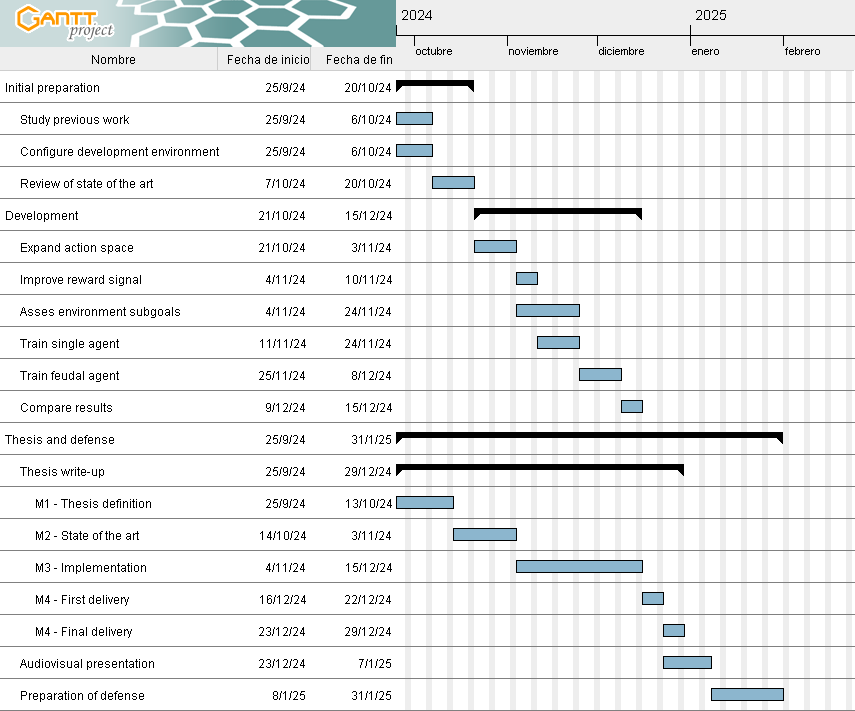
\includegraphics[width=.9\textwidth]{figs/TFM_Gannt.png}
    \caption[Gantt diagram of the planning for this project]{Gantt diagram of the planning for this project. Created with GanttProject\protect\footnotemark.}
    \label{fig:gantt}
\end{figure}
\footnotetext{\url{https://www.ganttproject.biz/}}

\begin{description}
    \item[Initial preparation] The first step of the project will involve studying and becoming familiar with the existing work that we will be using as a base, as well as setting up the development environment, which includes the tools mentioned in section \ref{section:tools}. Additionally, we will review the state of the art on relevant topics, such as hierarchical and feudal reinforcement learning.
    \item[Development] The development phase will take up most of the available time for the project. This is where we will try to achieve the goals laid out in section \ref{section:goals}. First will come the changes to the environment: the expansion of the action space and the improvement to the reward signal. After that, we will begin training the single agent to use as a benchmark. At the same time, we will study the environment in search of new subgoals. Finally, we will train the feudal agents and will compare the results of both strategies.
    \item[Thesis and defense] The process of writing the thesis document will be carried out in parallel to the development of the project and will follow a schedule of mandatory handouts---M1 to M5. Once the document is finished, we will move on to prepare the audiovisual presentation and the final defense.
\end{description}

\section{Report structure}

Next, we include a brief description of the future chapters of this report:

\begin{description}
    \item[Chapter \ref{chapter:state_of_the_art}] Presents an introduction to reinforcement learning and the state of the art of the techniques that we will use throughout the project.
    % TODO Complete
\end{description}